\documentclass[12pt]{article}
\usepackage{fullpage,enumitem,amsmath,amssymb,graphicx}

\begin{document}

\begin{center}
{\Large CS221 Fall 2018 Homework [scheduling]}

\begin{tabular}{rl}
SUNet ID: & prabhjot \\
Name: & Prabhjot Singh Rai
\end{tabular}
\end{center}

By turning in this assignment, I agree by the Stanford honor code and declare
that all of this is my own work.

\section*{Problem 0}

\begin{enumerate}[label=(\alph*)]
  \item The problem statement can be visualised as below: \\
  \begin{center}
  \includegraphics[scale=0.1]{IMG_2239.png}
  \end{center}
  \textbf{Variables}: The variables for the CSP are the m switches, $X_1, X_2 ... X_m$. The domain of these variables are Domains $   \epsilon \{0, 1\}$, $0$ being the "off" state for a switch and $1$ being the "on" state. \\
  \textbf{Constraints}: The constraints or the factors are created among a bulb and it's controlling switch(es). For example, from above Figure 1, if switch 1 controls bulb 1 and bulb 2, and switch 2 controls bulb 2 and bulb 3, a factor corresponding to bulb 1 would have switch 1 value as it's parameter (be dependent on switch 1) and bulb 2 would have values of both switch 1 and switch 2 as it's parameters. Since $T_j$ (for each button $j=1, ...m$) defines every set of light bulbs a switch controls, factor $f_k$ (for each light bulb $k=1,...n$) would depend on variable $j$ if $k$ in $T_j$. The value of this factor should return an odd number, so that even numbers render the state of the bulb to be "off" and last number makes the bulb "on".
  \begin{align*}
  f_k (X_1[\text{$k$ in $T_1$}], & X_2[\text{$k$ in $T_2$}], ... X_m[\text{$k$ in $T_m$}]) \\ & = sum(X_1[\text{$k$ in $T_1$}], X_2[\text{$k$ in $T_2$}], ... X_m[\text{$k$ in $T_m$}]) \% 2 == 1
  \end{align*}
  \item
  \begin{enumerate}[label=\roman*.]
  \item For finding consistent assignments, we draw the table for finding values of $t_1$ and $t_2$. From the Table 1, we can see that there are two consistent solutions for $x_1, x_2, x_3$, one being $\{0, 1, 0 \}$ and other being $\{ 1, 0, 1\}$, respectively.
  \begin{table}
\centering
\caption{Table depicting consistency calculation for XOR operation}
\begin{tabular}{|l|l|l|l|l|l|} 
\hline
x1 & x2 & x3 & t1(x) & t2(x) & \textbf{Consistency}  \\ 
\hline
0  & 0  & 0  & 0       & 0       & 0                     \\ 
\hline
0  & 0  & 1  & 0       & 1       & 0                     \\ 
\hline
0  & 1  & 0  & 1       & 1       & 1                     \\ 
\hline
0  & 1  & 1  & 1       & 0       & 0                     \\ 
\hline
1  & 0  & 0  & 1       & 0       & 0                     \\ 
\hline
1  & 0  & 1  & 1       & 1       & 1                     \\ 
\hline
1  & 1  & 0  & 0       & 1       & 0                     \\ 
\hline
1  & 1  & 1  & 0       & 0       & 0                     \\
\hline
\end{tabular}
\end{table}
  \item For fixed variables $X_1, X_2, X_3$, backtrack will be called in following ways:
  \begin{align*}
  backtrack(\phi, 1, \{x_1: [0, 1], x_2: [0, 1], x_3: [0,1]\}) \\
  backtrack(\{x_1: 0\}, 1, \{x_1: [0, 1], x_2: [0, 1], x_3: [0,1]\}) \\
  backtrack(\{x_1: 0, x_3: 0\}, 1, \{x_1: [0, 1], x_2: [0, 1], x_3: [0,1]\}) \\
  backtrack(\{x_1: 0, x_2: 1, x_3: 0\}, 1, \{x_1: [0, 1], x_2: [0, 1], x_3: [0,1]\}) \\
  backtrack(\{x_1: 0, x_3: 1\}, 1, \{x_1: [0, 1], x_2: [0, 1], x_3: [0,1]\}) \\
  backtrack(\{x_1: 1\}, 1, \{x_1: [0, 1], x_2: [0, 1], x_3: [0,1]\}) \\
  backtrack(\{x_1: 1, x_3: 0\}, 1, \{x_1: [0, 1], x_2: [0, 1], x_3: [0,1]\}) \\
  backtrack(\{x_1: 1, x_3: 1\}, 1, \{x_1: [0, 1], x_2: [0, 1], x_3: [0,1]\}) \\
  backtrack(\{x_1: 1, x_2: 0, x_3: 1\}, 1, \{x_1: [0, 1], x_2: [0, 1], x_3: [0,1]\})
  \end{align*}
  Therefore, backtrack algorithm is called 9 times.
  \item When lookahead is enabled (AC3):
  \begin{align*}
  backtrack(\phi, 1, \{x_1: [0, 1], x_2: [0, 1], x_3: [0,1]\}) \\
  backtrack(\{x_1: 0\}, 1, \{x_1: [0], x_2: [1], x_3: [0]\}) \\
  backtrack(\{x_1: 0, x_3: 0\}, 1, \{x_1: [0], x_2: [1], x_3: [0]\}) \\
  backtrack(\{x_1: 0, x_2: 1 x_3: 0\}, 1, \{x_1: [0], x_2: [1], x_3: [0]\}) \\
  backtrack(\{x_1: 1\}, 1, \{x_1: [1], x_2: [0], x_3: [1]\}) \\
  backtrack(\{x_1: 1, x_3: 1\}, 1, \{x_1: [1], x_2: [0], x_3: [1]\}) \\
  backtrack(\{x_1: 1, x_2: 0 x_3: 1\}, 1, \{x_1: [1], x_2: [0], x_3: [1]\})
  \end{align*}
  Therefore, backtrack algorithm with AC3 is called 7 times.
\end{enumerate}
\end{enumerate}
\section*{Problem 2}

\begin{enumerate}[label=(\alph*)]
  \item \textbf{Reducing the CSP:} In order to reduce an N-ary CSP to unary or binary factors, we can think of introducing another set of variables ($B_1$, $B_2$, $B_3$ and $S$) called auxiliary variables to keep a track of total sum of variables $X_1$, $X_2$ and $X_3$ as we traverse in the graph.\\ \\
  \textbf{Auxiliary variables introduction}: Following is the graphical representation of auxiliary variables $B_1$, $B_2$, $B_3$ and $S$ and given variables $X_1$, $X_2$ and $X_3$.
  \begin{center}
  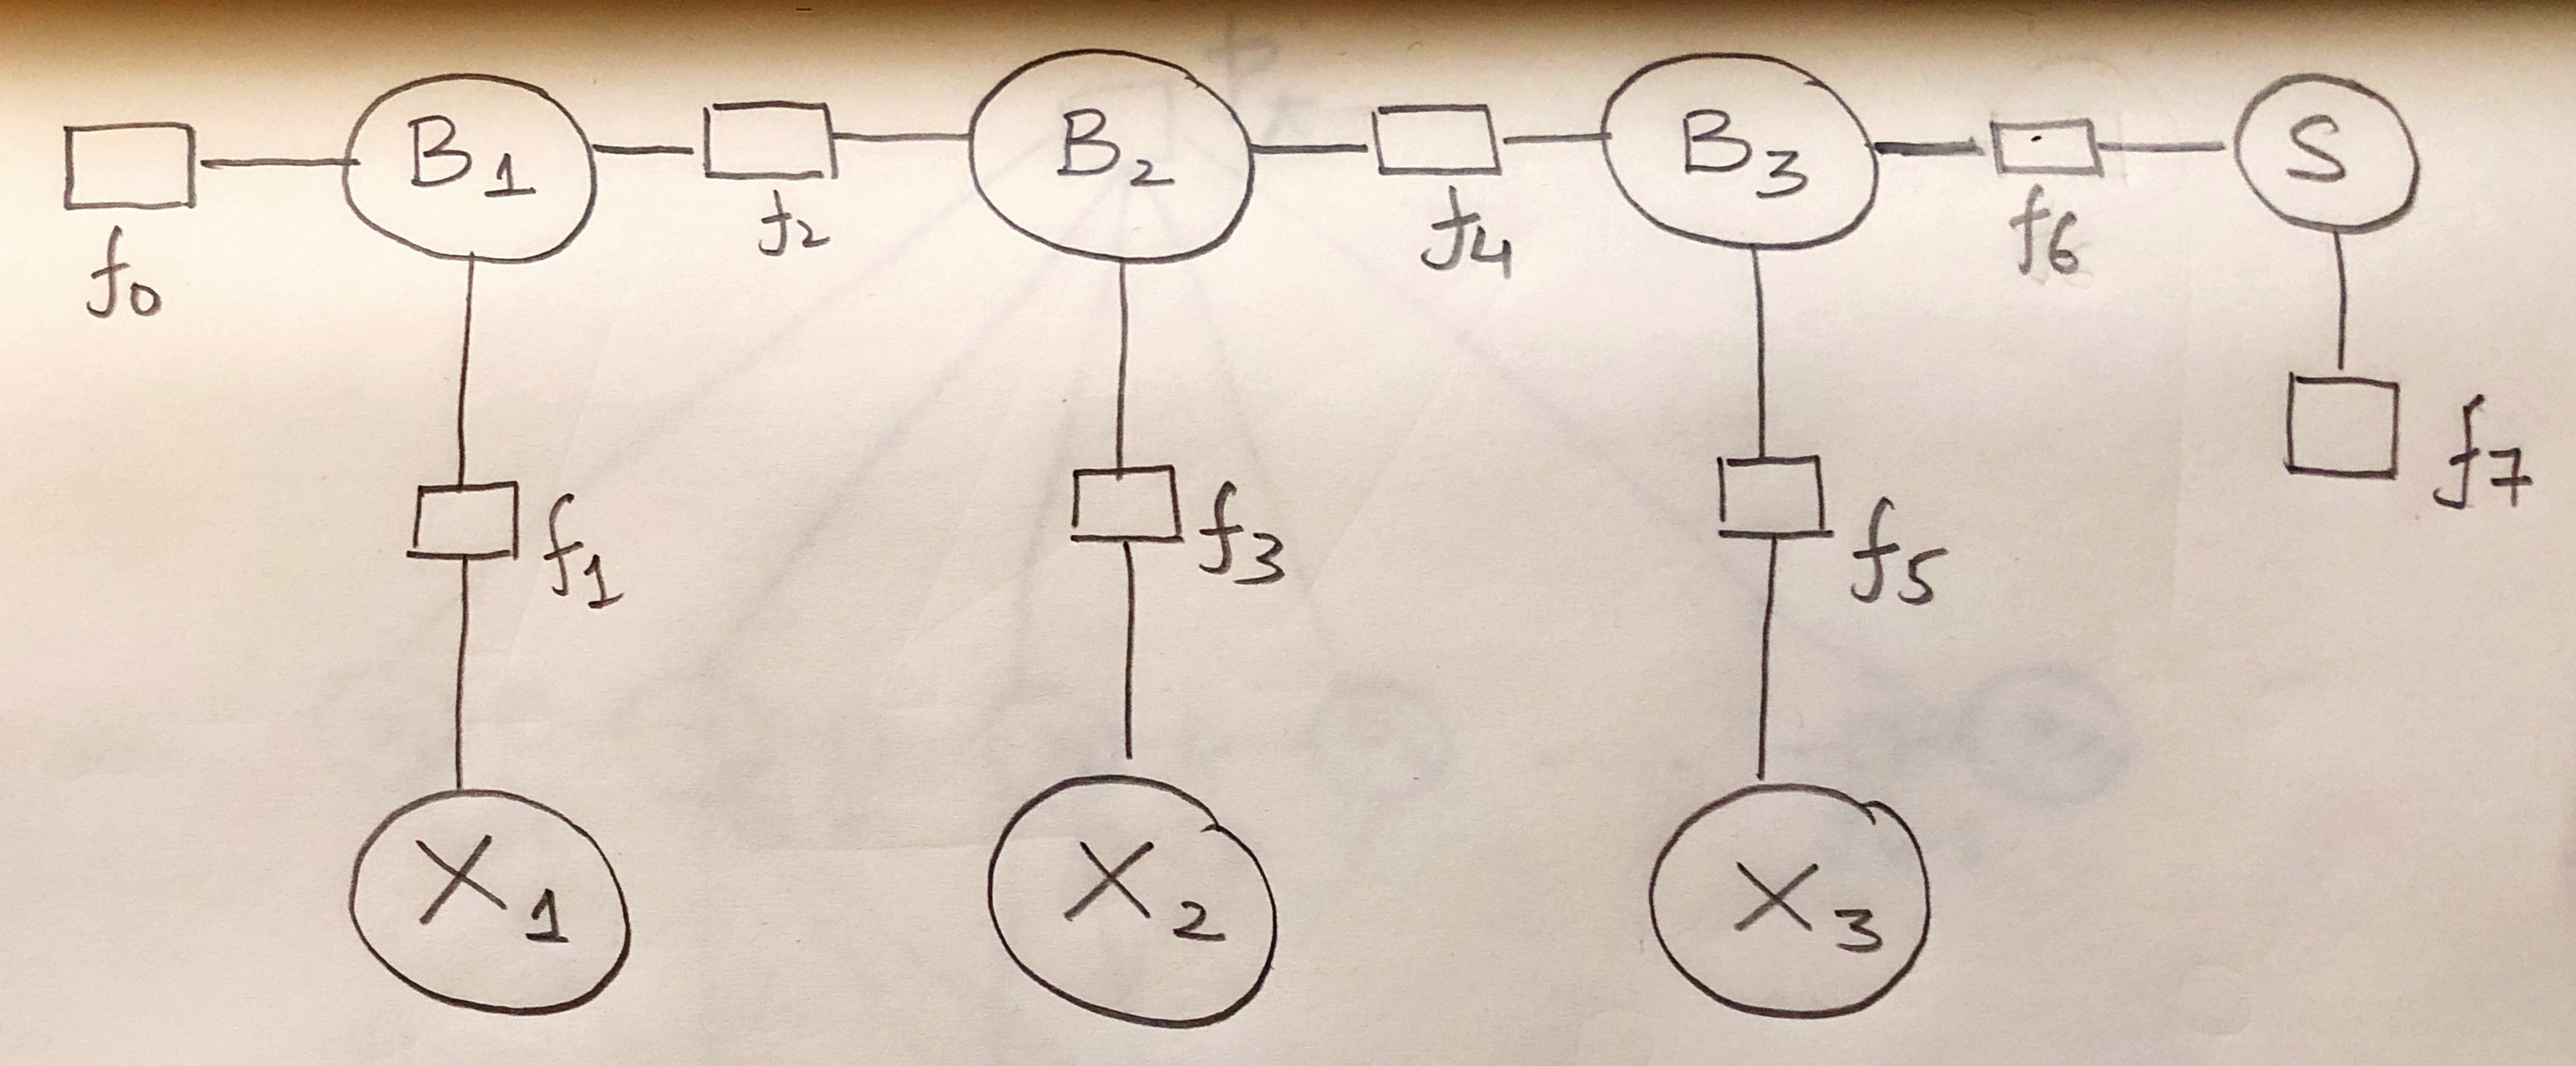
\includegraphics[scale=0.1]{IMG_2240.jpg}
  \end{center}
  \textbf{Domains}: $X_1$, $X_2$ and $X_3$ are the given variables with domains $\{0, 1, 2\}$ each. As discussed earlier, auxiliary variables $B_1$, $B_2$ and $B_3$ keep a track of the total sum. Therefore, these are two dimensional, one element carrying the total sum of previous auxiliary variable and other keeping a record after adding value of attached variable $X_i$. Both $B_n[0]$ and $B_n[1]$ will have a range from $0, 1, ... K$, where K being the maximum sum constraint. $S$ is the sum variable, having domain $0, 1, ... K$ since it tries to bind the variables based on given total sum. \\ \\
  \textbf{Constraints}: There are going to be unary and binary constraints as follows(referencing above image): \\ \\
  $f_0$ states that $B_1[0]$ should be 0, since we start with sum = 0. Therefore, $f_0(B1) = B_1[0] == 0$ \\ \\
  $f_1, f_3$ and $f_5$ make sure that adding $X_i$ to first coordinate of $B_i$ gives us second coordinate of $B_i$. Hence, $f_1(B_1, X_1) = B_1[0] + X_1 == B_1[1]$, similarly for $f_3(B_2, X_2) = B_2[0] + X_2 == B_2[1]$, and for $f_5(B_3, X_3) = B_3[0] + X_3 == B_3[1]$. \\ \\
  $f_2$ and $f_4$ make sure that first index of $B_{i+1}$ is equal to last index of $B_{i}$. Hence, $f_2(B_2, B_1) = B_2[0] == B_1[1]$ and $f_4(B_3, B_2) = B_3[0] == B_2[1]$. \\ \\
  $f_6$ maintains that last index of $B_3$ and the value of sum variable $S$ are equal. Therefore, $f_6(B_3, S) = B_3[1] == S$. \\ \\
  This scheme works because it has added maximum value constraint over the sum of all three variables through auxiliary sum variable $S$, along with propagating sum of variables one by one from $X_1$ to $X_3$ using $B_1$, $B_2$ and $B_3$.
\end{enumerate}

\section*{Problem 3}
\begin{enumerate}[label=(\alph*)]
\addtocounter{enumi}{2}
\item Since I am planning to pursue graduate certificate by taking up courses every quarter(except summer break), with propensity towards CS221 and CS224N, I listed out all the courses offered and let the system suggest what courses should I pick up when. Here's the profile I created: \\ \\
\# Unit limit per quarter. You can ignore this for the first \\
\# few questions in problem 2. \\
minUnits 3 \\
maxUnits 3 \\

\# These are the quarters that I need to fill. It is assumed that \\
\# the quarters are sorted in chronological order. \\
register Aut2018 \\
register Win2019 \\
register Spr2019 \\
register Aut2019 \\

\# Courses I've already taken \\
taken CS107 \\
taken CS103 \\
taken CS106X \\
taken CS106B \\
taken CS103 \\
taken CS124 \\

\# Courses that I'm requesting \\
request CS221 in Aut2018 weight 2 \\
request CS157 \\
request CS223A \\
request CS224N in Aut2019 weight 2 \\
request CS228 \\
request CS229 \\
request CS231A \\
request CS227B \\

The best schedule that the system suggested is depicted in Table 2. It makes sense because I had given higher weights to CS221 and CS224N, since I personally wanted to take these courses up with a vision to finish the graduate certificate as soon as possible. As I am working, I wanted to restricted the courses to 1 per quarter, therefore added maxUnits and minUnits for this profile as 3.
\begin{table}
\centering
\caption{Table Depicting best schedule suggested by system}
\begin{tabular}{lll}
Quarter & Units & Course  \\
Aut2018 & 3     & CS221   \\
Win2019 & 3     & CS223A  \\
Spr2019 & 3     & CS227B  \\
Aut2019 & 3     & CS224N 
\end{tabular}
\end{table}
\end{enumerate}

\section*{Problem 4}

\begin{enumerate}[label=(\alph*)]
\item If we were to include notable patterns as factors to CSP, the graph would look like the following:
  \begin{center}
  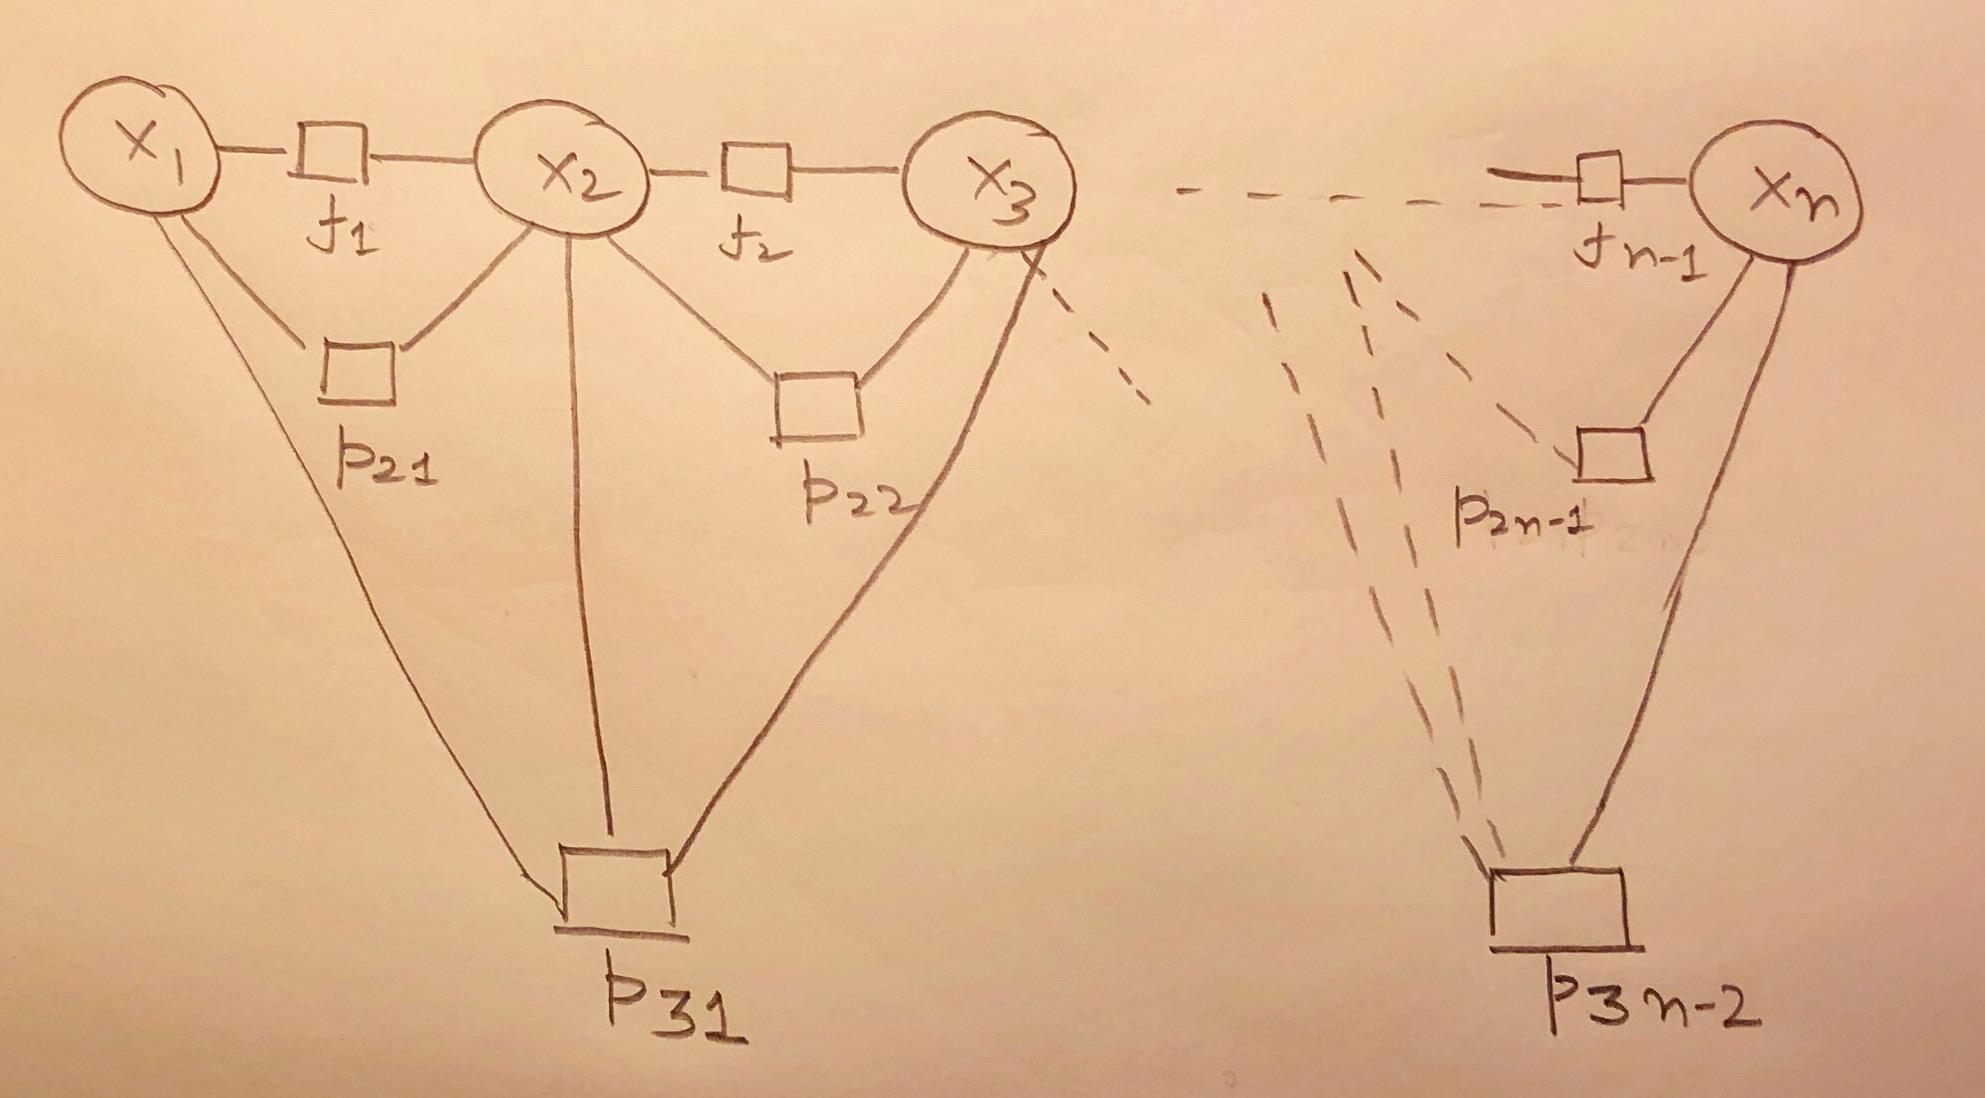
\includegraphics[scale=0.2]{IMG_2245.jpg}
  \end{center}
  where $X_1$, $X_2$ ... $X_n$ are variables, consecutive pairs connected by factors $f_1$, $f_2$ ... $f_{n-1}$. The notable patterns, when introduced as constraints, have arity based on the length of the pattern. For example, in the above image, one type of constraints are binary constraints($p_{21}$, $p_{22}$ ... $p_{2n-1}$) occurring over each consecutive pair, checking for existence of a sequence [x, y] being satisfied. Other type are ternary constraints occurring on all possible 3 consecutive variables($p_{31}$, $p_{32}$ ... $p_{3n-2}$). \\
  In worst case scenario would be a notable pattern constraint expecting all variables to take a particular value (meaning having length equal to number of variables). Tree width in this case would be $n$, since variable elimination cannot be done with any of the variables as the pairs are connected via multiple constraints.
  
  \item Let $p_t$ be the factors introduced by notable patterns. These are N-ary constraints, added to all sequences of variables. They have arity based on the length of the pattern(described in 4a). The algorithm would be as follows: \\ \\
  best\_weight = 0 \\
  best\_assignment = \{\} \\
  max\_weight\_assignment(x, f, n, Domains)
  
  \hspace{10mm}If x is complete assignment and $f \gamma^n$ is greater than best\_weight : 
  
  \hspace{20mm}best\_weight = $f \gamma^n$ and best\_assignment = x and return
  
  \hspace{10mm}Choose unassigned VARIABLE $X_i$ which has least consistent values
  
  \hspace{10mm}Order VALUES $Domain_i$ of chosen $X_i$ through least constrained value
  
  \hspace{10mm}For each value v in that order:
  
    \hspace{20mm}$\delta \leftarrow \pi_{f_j \epsilon D(x, X_i)} f_j(x \bigcup \{X_i: v\})$
    
    \hspace{20mm}If $\delta = 0$: continue
    
    \hspace{20mm}$N \leftarrow \sum_{p_t \epsilon D(x, X_i)} p_j(x \bigcup \{X_i: v\})$
    
    \hspace{20mm}Domains' $\leftarrow$ Domains via AC-2
    
    \hspace{20mm}max\_weight\_assignment($x \bigcup \{X_i: v\}, w\delta, n + N, Domains'$)
    
    max\_weight\_assignment(\{\}, 1, 0, \{ $X_1: [1,2...K]$, ..., $X_n: [1,2...K]$\})
    \\ \\
    The algorithm starts by checking if x(current assignment) is a complete assignment. If yes and the weight (which is $f \gamma^n$) is greater than best\_weight until that point, then it updates the current best\_weight and best\_assignment with $f\gamma^n$ and x respectively. Else, it continues and picks up an unassigned variable which has fewest consistent values(most constrained variable), and then picks up values based on least constrained value(order by least constrained value). Then for each value v it calculates the product of new factors $f_j$ which are dependent on the new assignment after $X_i = v$ is added to the existing assignment x. If $\delta = 0$, then we skip the current assignment else we continue and find out the value of N which is sum of the new notable pattern factors $p_j$ which are dependent on newly assigned variable. Furthermore, we update the domains via AC-3. And recursively call the max\_weight\_assignment function with new assignment, multiplying existing $f_i$ factors weight $f$ by $\delta$, add $N$ to observed sequences previously and with the updated domains via AC-3. The algorithm is initialised with empty assignment, 1 as factor weight of $f$, 0 as sum of notable patterns and original domain for every variable $X_i: [1,2...K]$. \\ \\
    
    Time complexity would be $O(K^n)$, since it can be visualised as a graph with depth $n$ and branching factor $K$. Space complexity would be $O(1)$ since we are not storing any variable with respect to the input size but just two constants, best\_weight and best\_assignment.
    
    
    
    

\end{enumerate}

\end{document}